\documentclass{standalone}
\usepackage{amsmath}
\usepackage{tikz}
\renewcommand{\familydefault}{\sfdefault}
\usepackage{bchart}

\begin{document}
% \begin{scope}
\begin{tikzpicture}
\node at (0, 0) {
\includegraphics{m1.png}}; 
\end{tikzpicture}

\begin{bchart}[max = 1, scale = 1, width = 2cm]
    \bcbar[label=man, color = blue!50]{0.88}
    \smallskip
    \bcbar[label=woman, color = red!50]{0.12}
\end{bchart}
\quad\quad\quad\quad
\begin{tikzpicture}
\node at (0, 0) {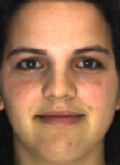
\includegraphics{w1.png}}; 
\end{tikzpicture}
\begin{bchart}[max = 1, scale = 1, width = 2cm]
    \bcbar[label=man, color = blue!50]{0.02}
    \smallskip
    \bcbar[label=woman, color = red!50]{0.98}
\end{bchart}

\end{document}